\section{Motivations}

In this section, we discuss the major motivations for creating NetStar.

\subsection {Callbacks vs Promises}

Currently, when writing NF code, the only method to handle asynchronous operations is to use callbacks: if the NF would like to query the database or the DNS server to retrieve important information, it has to send out the query first and register a callback function. When the response of the query arrives, the NF application should appropriately invoke this callback function and passes in the response. 

There has been a long lasting discussion about whether programmer should write callback functions to deal with asynchronous operations or use advanced programming techniques like promises \cite{}. The dominant conclusion is that using promise can significantly reduce application development effort by reducing the source code line count and maintaining a neat control flow.

Besides simple stateless packet transformers such as IP TLL adjuster and L2 switch, there is complicated NF software that needs to constantly perform asynchronous operations. Therefore, we believe that bringing promise into NFV development to address both flow and request-level asynchrony is important for NFV development as well.

Even though promises bring apparent advantages over callback functions, people rarely use promises to develop NF software. The primary reason is due to the complexity for supporting promises. Promise has a monadic structure \cite{} and requires that the implementing language has a strong type system to support generic type arguments, type deduction and first-class lambda function. For a long time, promises are only seen in functional programming languages like OCaml \cite{}, F-sharp \cite{} and Haskell \cite{}. These functional programming languages are not suitable for developing performance-sensitive NF software, as they all use GCs to reclaim unused memory resources and may incur unexpected program pause during the GC process.


In recent years, C++ \cite{} has evolved into a system programming language that supports a wide range of high-level features that are only seen in functional programming languages. Several promise implementation \cite{} is available in C++, including std::promise and boost::promise.


\section{Misc}

Our primary motivation for this paper comes from a recent advancement in building stateless network function. Stateless network function achieves dynamic scaling and fault tolerance, two of the most important topics that are active explored by network middlebox research community, by storing important flow states, including per-flow state or shared state, in a key-value store called RamCloud. In the most extreme cases, stateless network function needs to access the key-value store for every other packet that it processes.

Figure~\ref{fig:base-class} shows two implementation of a IPS system in StatelessNF. We can see that NetStar has an easier implementation, with smaller number of lines of code, preserved control flow, smaller number of defined functions, and better error handling code.

\begin{figure}[!t]
	\begin{subfigure}[b]{\columnwidth}
		\centering
 	 	\lstset{language=C, numbers=left, showspaces=false,
    		showstringspaces=false, tabsize=2, breaklines=true,
    		xleftmargin=5.0ex, basicstyle=\scriptsize,
		}

		\begin{lstlisting}
      class flow_context{
        async_flow<TCPType> _af;
        net::packt _cur_pkt;
        future<> run(){
          _af.on_new_packet().then([]{
            _cur_pkt = _af.get_packet();
            if(!_cur_pkt){
              return make_ready_future<>();
             }
            return mica_ready(flow_key);
          }).then([this](mica_query_response automaton state){
            auto new_state = automaton.check(_cur_pkt, state);
            if(new_state == alarm){
              drop(_cur_pkt);
              return make_ready_future<>();
             }
             else{
               return mica_write(flow_key, new_state);
             }
          }).then([](mica_query_response){
            return run();
          });
        }
       }
		\end{lstlisting}
		\caption{IPS implementation based on NetStar.}
		\label{fig:api}
    \end{subfigure}\hfill
	\begin{subfigure}[b]{\columnwidth}
		\centering
 	 	\lstset{language=C++, numbers=left, showspaces=false,
    		showstringspaces=false, tabsize=2, breaklines=true,
    		xleftmargin=5.0ex, basicstyle=\scriptsize,
		}

		\begin{lstlisting}
void on_first_pkt(context* ctx, packet* pkt){
  flow_tuple tp = extract_flow_tuple(pkt);
  automaton_state a_st = init_automaton_state();

  async_write_db_with_cb(ctx, tp, a_st, subsequent_pkt_read);
}

void subsequent_pkt_read(context* ctx, packet* pkt){
  flow_tuple tp = extract_flow_tuple(pkt);
  async_read_db_with_cb(ctx, tp, subsequent_pkt_write);
}

void subsequent_pkt_write(context* ctx, packet* pkt, automaton_state* a_st){
  char* next_byte = get_next_payload_byte(pkt);

  while(next_byte != nullptr){
    a_st = process_with_automaton(next_byte, a_st);
  }

  async_write_db_with_cb(ctx, tp, a_st, call_send_pkt);
}

void call_send_pkt(packet* pkt, context* ctx){
  send_pkt(pkt);
  update_ctx(ctx, subsequent_pkt_read);
}
		\end{lstlisting}
		\caption{A callback based implementation for stateless IPS.}\label{fig:example}
	\end{subfigure}
\caption{The API and implementation of an example NF module.}
\label{fig:base-class}
\end{figure}

\section{The Asynchronous Flow Abstraction}

\begin{figure}[!t]
  \centering
  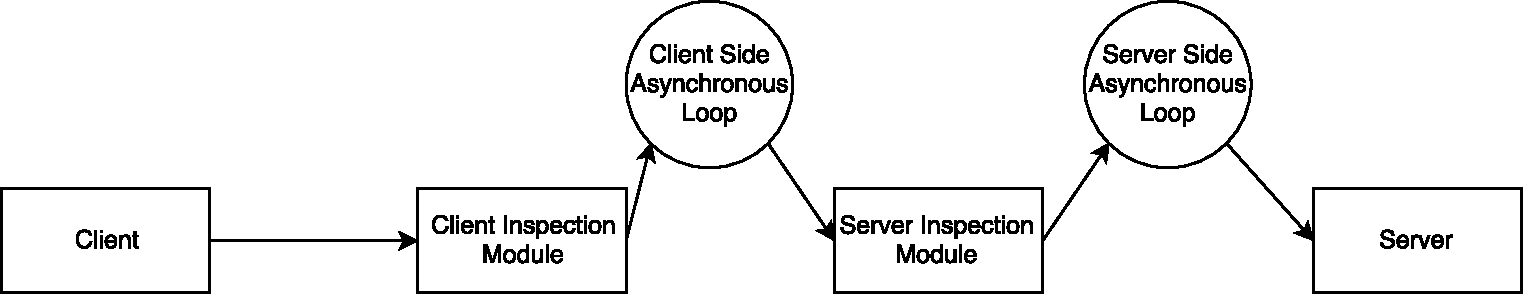
\includegraphics[width=\columnwidth]{figure/async-flow.pdf}
  \vspace{-2mm}
  \caption{The general-purpose asynchronous flow abstraction used in NetStar.}
  \label{fig:async-flow}
  \vspace{-6mm}
\end{figure}

Figure~\ref{fig:async-flow} illustrates our general purpose asynchronous flow abstraction used in NetStar. It is designed to process and inspect connection-oriented flows. It consists of four pluggable part. The client side inspection module aims to mimics the client protocol state. The client side asynchronous loop executes various asynchronous operations. The server side inspection module mimics the server side protocol state while the server side asynchronous loop executes various asynchronous operations as well. The server side asynchronous loop is capable of reconstructing the protocol payload (TCP payload) and analyzing the TCP pay load.

The four parts are pluggable. Programmer can disable uninterested part, making it fully modular. It is designed by combining the Seastar server side programming interface with mOS TCP/IP monitoring sock.
